\documentclass[11pt,a4paper]{article}
\usepackage{times}
\usepackage{fancyhdr}           % Allows better control over headers and footers
%\usepackage{layout}            % use with \layout to see the page layout for
%debugging purposes.
\usepackage[margin=2.5cm]{geometry}  %   set the margins using the
                                %   geometry package (which is much
                                %   the easiest way of doing this).
\usepackage[pdftex]{graphicx}   %   Pictures (means you have to
                                %   produce pdf output via pdflatex)
\usepackage[small,compact]{titlesec}   % Try to reduce the white space
                                % latex loves so much
\titlelabel{\thetitle. \quad}   % Reduce space around section heads
                                % and add a full stop after the number
\pagestyle{fancy}               % Invoke fancy headers

\renewcommand{\abstractname}{\vskip -5mm}  %  Change name of Abstract
                                %  to nothing and loose some of the
                                %  excessive white space
\newcommand{\itab}[1]{\hspace{0em}\rlap{#1}}
\newcommand{\tab}[1]{\hspace{.2\textwidth}\rlap{#1}}

\begin{document}
    \begin{titlepage} \begin{center}
            \textsc{\LARGE University of Cape Town}
            \\[1.5cm] \textsc{\Large Software Engineering Stage Four} \\\smallskip
            \textsc{\Large Final Report} \\\smallskip
            \textsc{\Large CSC3003S} \\\smallskip
            \textsc{\Large \today} \\\smallskip
            \noindent\rule[0.4mm]{\textwidth}{0.1mm}
            \\[0.4cm] { \huge \bfseries Tempest Trace \\[0.4cm] }
            \noindent\rule[0.4mm]{\textwidth}{0.1mm}
            \\[1cm]
            \begin{minipage}[t]{0.4\textwidth}
                \begin{flushleft}\large \emph{Authors:}\\ Brian Mc George - MCGBRI004 \\ Jacques Heunis - HNSJAC003 \\ Timothy Gwynn - GWYTIM001
                    \\[2cm]
                \end{flushleft}
            \end{minipage} \begin{minipage}[t]{0.4\textwidth}
            \begin{flushright} \large \emph{Supervisor:} \\ Assoc. Prof.~Patrick Marais\\patrick@cs.uct.ac.za\end{flushright}
            \begin{flushright} \large \emph{Tutor:} \\ Codie Roelf\\Codie.Roelf@alumni.uct.ac.za\end{flushright}
        \end{minipage}
    \end{center}
\end{titlepage}
\newpage
\tableofcontents
\newpage

%%%  Set the headers via fancyhdr package
\lhead{Capstone Project 2015}  % Short title for running head
\chead{}
\rhead{\today}   %  Fixed running head of the date
\lfoot{}
\cfoot{\thepage}    %  add page number as centre footer.
\rfoot{}
\renewcommand{\headrulewidth}{0.0pt}   % Don't want horizontal line
                                % under header.

\begin{abstract}
 The Tempest Trace project is focused around providing a two player, parkour game. Players race against each other to reach the final goal in a competitive 1st person runner game. Players must move over, under, around and through obstacles efficiently while avoiding enemy AI elements such as flying drones and snipers. An aspect that the game focuses on is allowing the player to choose from a variety of possible routes to gain advantage over his/her opponent; certain routes will be better in different situations so every race requires new strategies.  Players must choose the most efficient route to reach the end goal using their parkour skills ahead of their competitor. The aesthetic is purposefully simplistic and clean to allow the player to focus on gameplay and easily identify obstacles and objects to interact with. Players are also able to interact with the world and each other in order to gain a competitive advantage by slowing their opponent down in a variety of ways. In parkour flow and smoothness of movement are imperative and this is reflected in Tempest Trace, the shortest path is often not the fastest and maintaining movement is often more important than achieving the highest speed.
\end{abstract}

\section{Introduction}
The capstone project is done as the culmination of your three year
study of Computer Science. It is the development of a real application
that draws on all your knowledge of the field gained in the course of
your training in the subject.

The project should be written up as a professional software
engineering design and development project. We expect a report of
about 3500-4000 words, written single spaced, with a font size of at
least 11 pts. Use at least a 2.5 cm margin on all sides of the
pages. Please use ``styles'' for formatting if you are using a word
processing package or use \LaTeX. We mean you to use styles for
everything, not just headings and lists but also for a different
font. So use emphasis for \emph{italics} and do \emph{not} use a bold
face. No blank lines between paragraphs except to get figures and
their captions to position properly.

Depending on how many diagrams you use (more is better) the report
will be between 7 and 10 pages long. Note that while word users will
struggle with numbered headings and lists, \LaTeX\/ has its own ideas
about where ``floats'' (like tables and figures) will go, as usual
search the internet for advice (e.g., search for ``\LaTeX quick
guide'' and look at
http://www.andy-roberts.net/writing/latex/floats\_figures\_captions). Don't
worry, word's specialty is loosing your figures in some between-page
limbo; \LaTeX\/ will not loose them, just place them way after the
spot where you want them.  This document shows the format we expect
and you can use it as a template.  Your appendices (e.g., user manual,
test results, which are needed) are not included in these limits.

You must had-in an Adobe Acrobat file for your report (i.e., pdf
file). Not word, latex source, but \emph{PDF}!

\section{Approach}

You should begin your write-up with an overview and then drill down
into the details of what you produced. Your report should cover the
following sections (Sections \ref{ss:introduction} --
\ref{ss:conclusion}).

\subsection*{Abstract}
First you should have an executive summary (or abstract) just a single
paragraph saying what the results of the project are (at most 200
words).

\subsection{Introduction}
\label{ss:introduction}

Your introduction provides the context for the project and should
contain the statement of the scope of the project (which may have
changed since you first wrote it). Someone reading your introduction
must have clear idea of what the system is intended for. If you think
there is something special about the kind of problem you tackled that
your reader needs to know up front then this is where you say it.

If you need any survey of other work (you probably don't) then put it
towards the end of the introduction and give suitable references. A
case where this is needed is if your project builds on someone else's
project or some published algorithm.

Discuss your approach to solving the problem. Please give a short
overview of the software engineering methods you used (e.g.,
traditional analysis followed by design and implementation -- typically
the case if you did an evolutionary prototype, or a more agile
approach where you had a cyclical development process). 

\subsection{Requirements Captured}

The next section deals with the analysis of your system. Cover the
functional, non-functional and usability requirements. This is where
you present your use case narratives and diagrams. 

Discuss the major analysis artefacts that you produced. We will expect
you to produce at least one overall description of the architecture
used in your system as a diagram, either here or below (see Section
\ref{ss:design-overview}). You may also want to include an analysis
class hierarchy diagram.

\subsection{Design Overview}
\label{ss:design-overview}

The next section is an overview of your design. The system design has
to be justified in terms of the expected behaviour of the final
product. 

If you produced a design class diagram put it here.

\begin{figure}[h!]
  \center{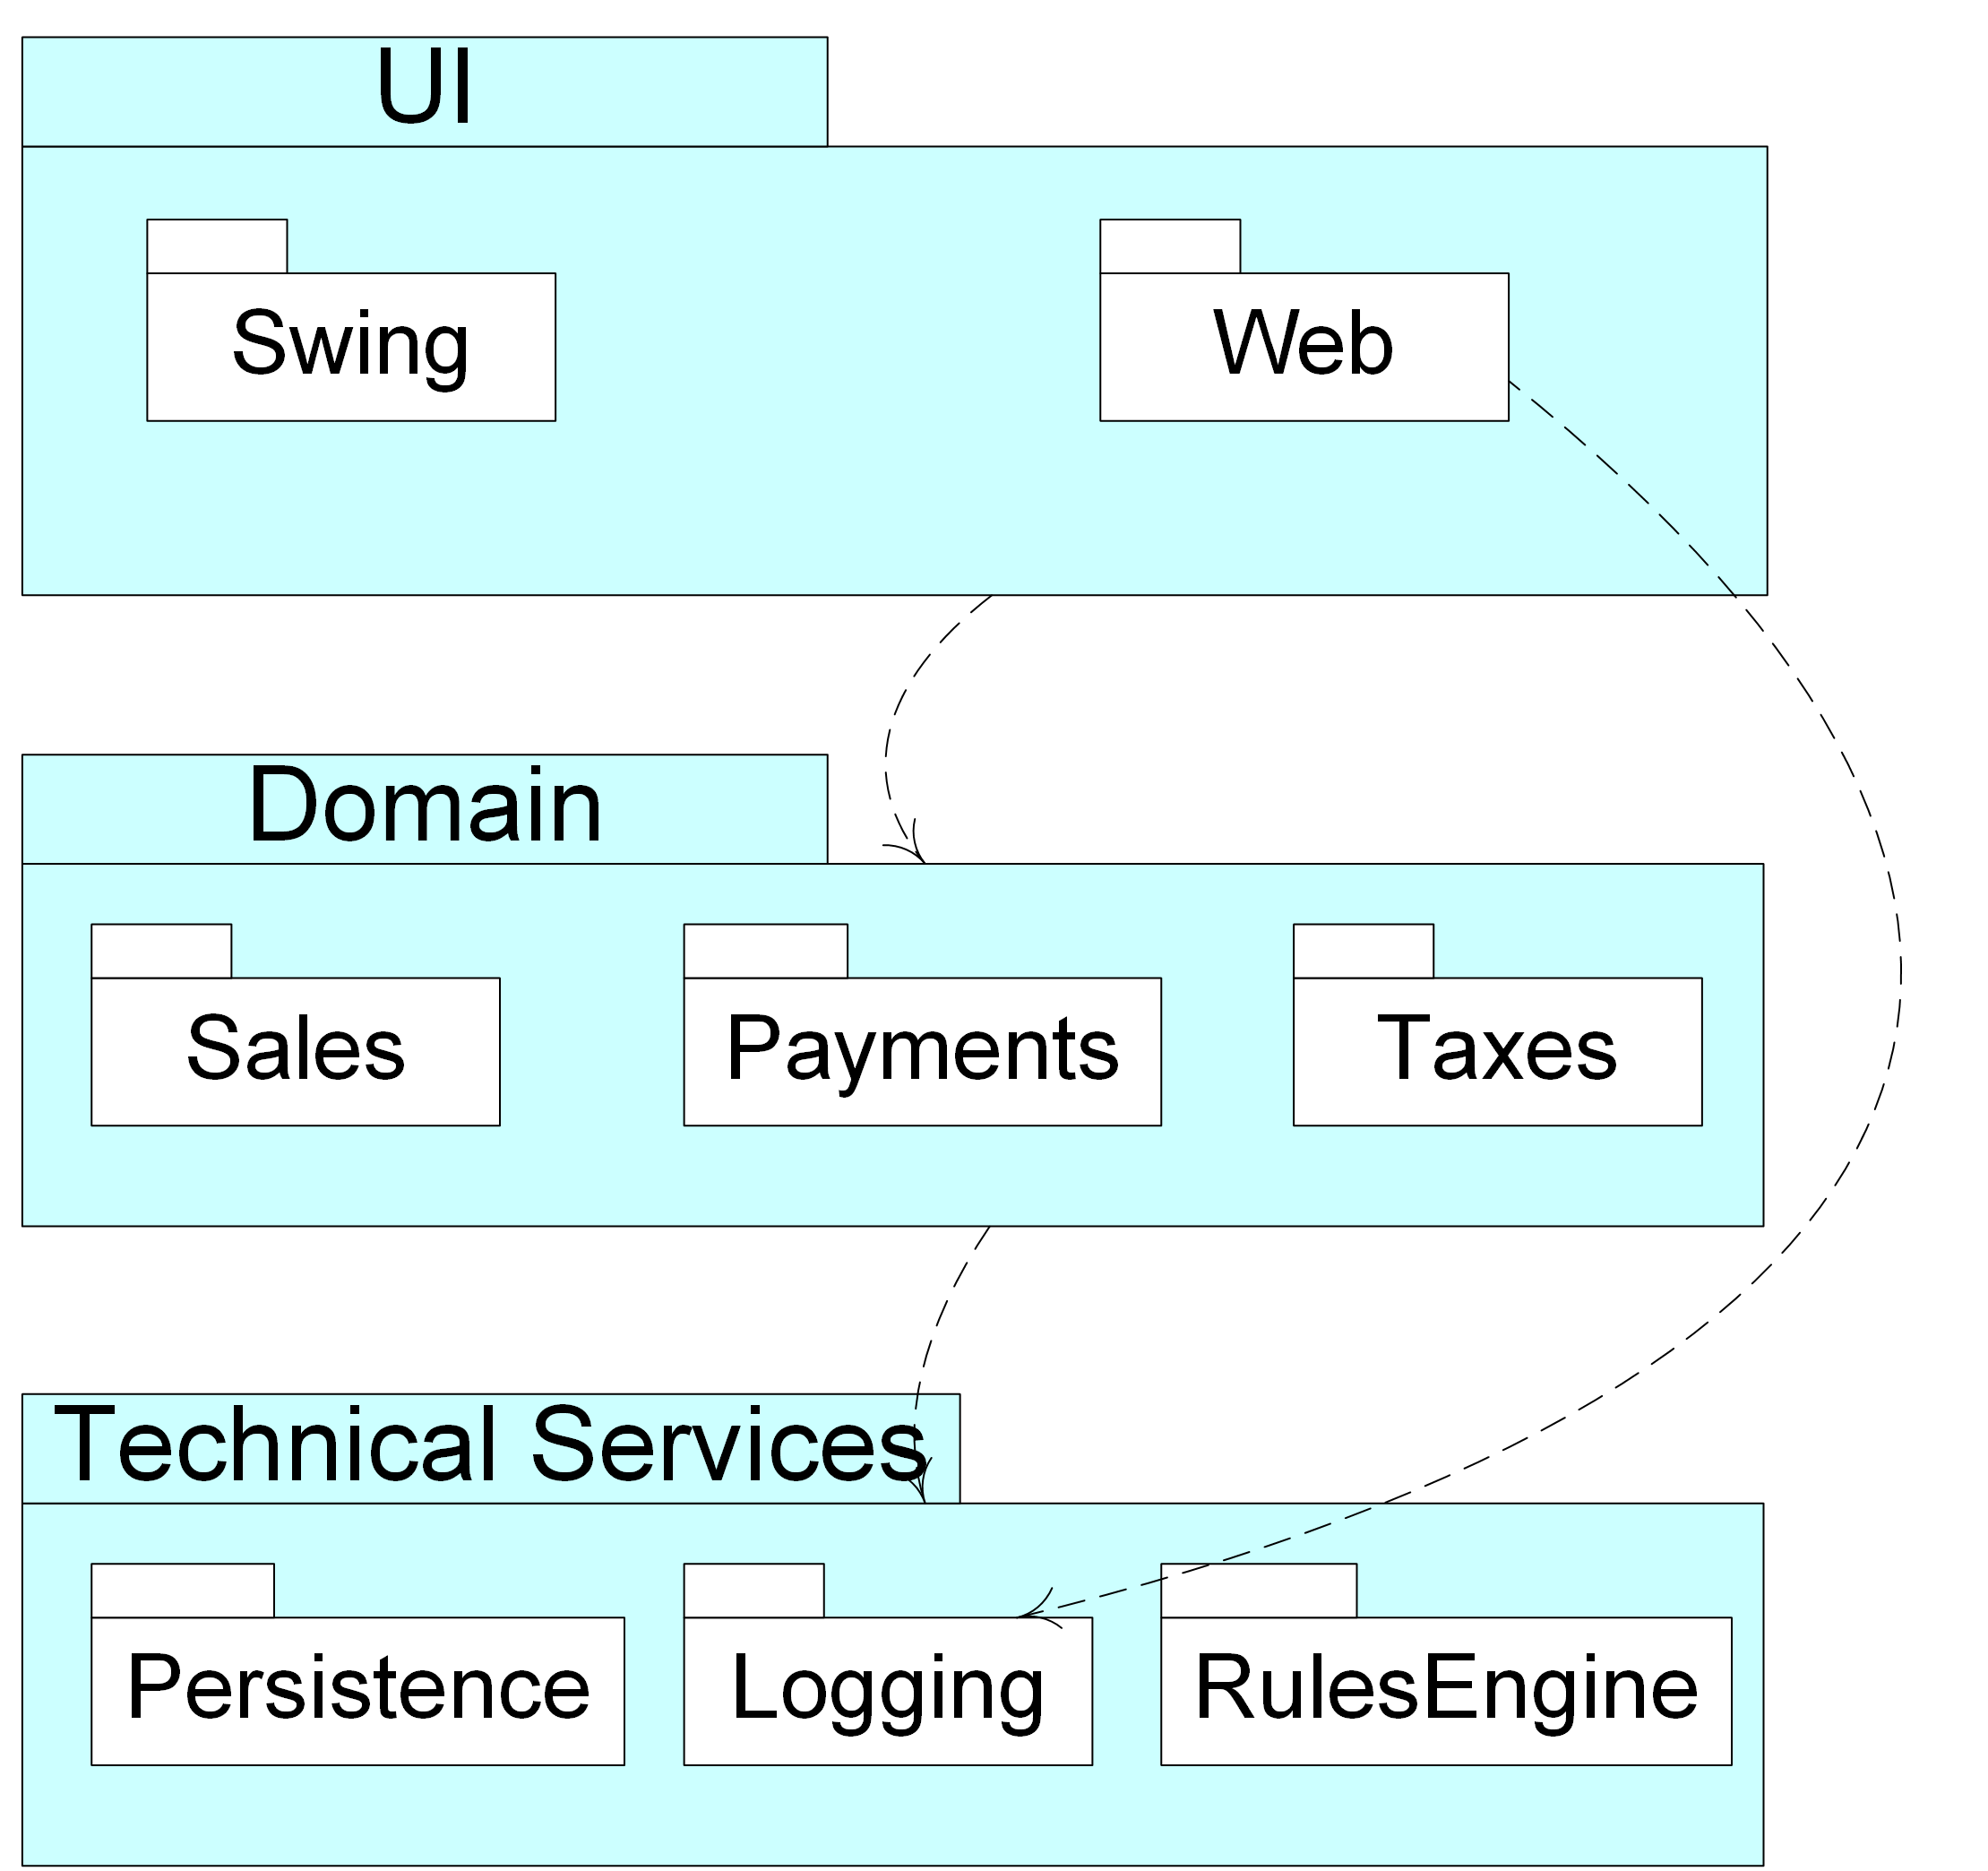
\includegraphics[scale=0.8]{architecture.png}}
  \caption{An architecture diagram. Caption to go below figure}
  \label{fig:architecture}
\end{figure}

You must present the overall architecture of the system together with
an architecture diagram. You may choose what kind of diagram best
suits your project but we would expect a layered architecture diagram
(see Figure \ref{fig:architecture}) unless there is a good reason for
some other kind of diagram. It need not be a formal UML diagram as
long as it conveys all the necessary information clearly.

You should then (in subsections) cover the algorithms and the data
organisation used and why they were considered the best. 

\subsection{Implementation}

Now we get to the details. 

\begin{itemize}
\item Describe your data structures and be sure to illustrate them
  with a diagram.

\item If your user interface was a key feature describe how that was
  implemented.

\item Discuss the function of the most significant methods in each
  class. This may well require flowcharts, or sequence diagrams, in
  some cases.

\item Any special relationship between the classes (e.g. friends) and
  why they exist.

\item A description of any special programming techniques or libraries
  used.
\end{itemize}

\subsection{Program Validation and Verification}
\label{ss:progr-valid-verif}

Tell us how you tested the system and why you believe it works.
Describe the Quality Management Plan for your project, that is,
software testing plan. The plan should indicate the types of testing
that was performed and detail how they were done. This must include
the reasons on why the chosen testing protocol was considered
effective.

Create a table that summarizes the testing plan (see Table
\ref{tab:test-plan}).

\begin{table}[h!]
  \centering
\caption{Summary Testing Plan. A table caption goes above the table.}

\begin{tabular}[t]{|p{8cm}|p{7cm}|} \hline

  \textbf{Process} & \textbf{Technique} \\ \hline 1. Class
    Testing: test methods and state behaviour of classes & Random,
    Partition and White-Box Tests \\ \hline 2. Integration Testing:
    test the
    interaction of sets of classes & Random and Behavioural Testing \\
    \hline 3. Validation Testing: test whether customer requirements
    are satisfied & Use-case based black box and Acceptance tests \\
    \hline 4. System Testing: test the behaviour of the system as part
    of a larger environment & Recovery, security, stress and
    performance tests \\ \hline

\end{tabular}

\label{tab:test-plan}
\end{table}
Describe all the steps taken to validate the correctness of the
program.

If you had user tests then say what you did and what the results
were. Describe why these test data were chosen (what test conditions
the data was testing).  Table \ref{tab:tests} provides an example of
the sorts of results we are looking for. The full detail of the test
runs should be appended to the report.

\begin{table}[h!]
  \centering
\caption{A table of tests. A table caption goes above the table.}

  \begin{tabular}[t]{|p{5.5cm}|p{3cm}|p{3cm}|p{3cm}|} \hline \textbf{Data Set
    and reason for its choice} & \multicolumn{3}{c|}{\textbf{Test Cases}}\\
    \cline{2-4} & \emph{Normal Functioning} & \emph{Extreme boundary cases} &
    \emph{Invalid Data (program should not crash)} \\ \hline Preliminary test
    (see Appendix 3) & Passed & n/a & Fell over \\\hline &&&\\ \hline
    &&&\\ \hline
  \end{tabular}

\label{tab:tests}
\end{table}

Follow your table of results with a discussions of them highlighting
how useful and usable your system is for its intended purpose.

\subsection{Conclusion}
\label{ss:conclusion}

Your report must have a clear conclusion where you revisit the aims
set out in the beginning and discuss how well you met them. Did you
achieve the objective of creating a well-structured, modular, and
robust system?  Please summarize the design features and test results
that show this.

\subsection{User Manual}
\label{ss:user-manual}
\begin{description}
	\item [Goal] Get to the top of the last building before the other player. Move quickly and efficiently while avoiding danger from enemies and falls.
	\item [Enemies] Flying drones will attempt to chase you down if you get too close to them. Snipers will shoot you if you expose yourself in their field of vision.
	\item [Enviroment] Interact with objects such as doors and buttons in your enviroment by pressing the object interaction button. Buttons will often let you gain a tactical advantage over your oponent.
	\item [Player 1 Controls]\hfill \\
	\begin{description}
		\item \itab{Look:}\tab{Mouse}
		\item \itab{Movement:}\tab{WASD}
		\item \itab{Jump:}\tab{Spacebar}
		\item \itab{Slide:}\tab{Shift}
		\item \itab{Somkebomb:}\tab{F}
		\item \itab{Object Interaction:}\tab{E}
	\end{description}
	\item [Player 2 Controls]\hfill \\
	\begin{description}
		\item \itab{Look:}\tab{Right Joystick}
		\item \itab{Movement:}\tab{Left Joystick}
		\item \itab{Jump:}\tab{Left Bumper}
		\item \itab{Slide:}\tab{Right Bumper}
		\item \itab{Somkebomb:}\tab{B Button}
		\item \itab{Object Interaction:}\tab{A Button}
	\end{description}
\end{description}
Your system must have a user manual. Append this to your report (make
it Appendix A) or bind it separately if it is big. If your system is
interactive and has a good user interface with context dependent help
then this can be just a cheat sheet. Discuss the level at which your
user manual is to be pitched with your client. If your system is to be
extended then you might want to include a technical API manual.

\section{Conclusion}
\label{sec:conclusion}

This document has covered the major sections needed for your
report. You will probably have each of the subsections 2.1--2.7 as
major section in the report each with its own subsections. 

A marking guide for the report will be provided later.

\appendix
\section{Code Legibility and Output}

This is not strictly part of the report but is a requirement for the
final hand-in.

\begin{itemize}
\item Each method should start wide a brief description of its
  function.

\item Use indentation to display the structure within a method.

\item Comments should be used extensively. They are best used to
  describe logical blocks of code rather than individual
  statements. Line-by-line comments have the drawbacks of not
  providing any overview and of decreasing readability.

\item Meaningful identifiers should be chosen.

\item Output should be pleasingly formatted and easy to read.
\end{itemize}

You do, of course, have the option to call in any of your
favourite packages for setting maths, graphics, computer listings,
etc.

\begin{thebibliography}{9}

\bibitem[Kopka and Daly(2004)]{KopkaDaly}
Kopka, H. and Daly, P.W.  (2004) \textit{A Guide to \LaTeXe:
Document Preparation for Beginners and Advanced Users} (4th~edn).
Addison-Wesley.

\bibitem[Lamport(1994)]{Lamport}
Lamport L. (1994) \textit{\LaTeX: A Document Preparation System}
(2nd~edn). Addison-Wesley.

\bibitem[Mittelbach and Goossens(2004)]{Companion}
Mittelbach, F. and Goossens, M., (2004) \textit{The \LaTeX\
Companion} (2nd~edn). Addison-Wesley.

\end{thebibliography}
\end{document}
